\chapter{Providing Information}
\begin{flushright}
    \textit{``Science, done right, is one of the humanities.''}
    \\ --- Daniel C. Dennett
\end{flushright}

On a train station platform in Auckland, NZ, there is a florist. This florist has a till, sticky taped to this till is a sign, a homemade sign by somebody who's quite good at Word, `cos they flipped the sign into landscape. On the sign in bold letters, it says:

\begin{center}
\textbf{NO INFORMATION \\ PROVIDED}
\end{center}

What is \textit{THAT!?} That sign may well have just said, `I HATE EVERYONE!' What sort of fact hoarding monster is this? Do they expect to defend their life in a competitive game of trivial pursuit? At the time, I was midway through buying some flowers, and I asked the florist what that sign meant, and she said to me in quite a pompous tone of voice \textit{``It means... we don't provide information"}. I had to resist my ninja-like comedic instincts to say \textit{``well... let's cast our minds back to what literally just happened"}. Instead, I asked her what kind of information do they not provide, to which she said, \textit{``you know... where things are, what time the train leaves, where the toilets are... stuff like that"}. Where the toilets are!? She refuses to point out amenities to the people who might desperately need them? Would she refuse to locate the handicap access to the disabled? Would she refuse to locate the station's defibrillator to a person in cardiac arrest? This woman was genuinely telling me that if if a 47-year-old businessman runs to her, sweat on his brow, blood on his shirt, eyes dancing with the terror of an infant, frantically spluttering: \textit{``quick, help me, please, I've been stabbed, where is the first aid kit?"}, she would willing choose to say \textit{``Oh-no-no-no... read the sign... bleed quietly... and learn your lesson."}


% \footnote{The location of publicly accessible defibrillators in NZ: \url{https://aedlocations.co.nz/}}.

% How dire does a situation need to be for her to break her solemn vow and provide information to those who ask? 

% \textit{``Oh-no-no-no... read the sign... shit your pants... learn your lesson."}

% \textit{``you know...where hotels are, what time the train leaves, where the toilets are... things like that"}. Where the toilets are!? She refuses to tell people where toilets are!? Are we not all fundamentally at some basic level, septic tanks on legs trying not to shit themselves? I'm sure everybody at some point in their dignified adult lives has thought, \textit{``oh dear me. I need to poo... much sooner than I had hoped"}. This woman was genuinely telling me that if a 47-year-old businessman runs to her, sweat on his brow, eyes dancing with the terror of an infant, frantically spluttering: \textit{``quick, help me, please help me, quickly, where are the toilets?"}, she would willing choose to say \textit{``Oh-no-no-no... read the sign... shit your pants... learn your lesson."}

I understand the exasperation at the world that leads one to put that sign up. We have all, at some point in our lives, felt the frustration of other people and the lure of isolation. We've looked at the world and seen it for what it is, and the one reasonable response is to not want to be a part of it. But to have that feeling, and to go home and laminate that feeling, are two different things. Of course, it is easier to refuse to provide information to someone. It's easier not to engage with other people's lives and their problems because oftentimes their problems will contradict your own. The very things that cause them pleasure bring you pain. Why would you help someone else when they are clearly the problem with your world. Rich people blame the poor; poor people blame the rich; old people blame the young; young people blame the old; left-wing liberals and right-wing conservatives blame each other; atheists and fundamentalists blame each other; vegans and carnivores blame each other; genders blame each other; races blame each other; car drivers and bike riders blame each other, tea drinkers and coffee drinkers ---it's about time that fight kicks off. Surely the one conclusion we can draw from this equation of deferred responsibility is that we are all fundamentally, to a greater or lesser degree, the problem with the world, though we rarely admit it. It's too easy to fall into the trap of looking out your metaphorical window at the world and reaching the conclusion that the problem with the world are people that aren't you. Right now, I'm wearing slippers and have just made myself a sandwich. It's difficult for me to see exactly how those actions bring harm to the world. 

It is a betrayal to deny someone information. Surely it is our duty as people to pool every drop of information we have and collectively hurl ourselves at the stars.

\vspace{5mm}
\begin{center}
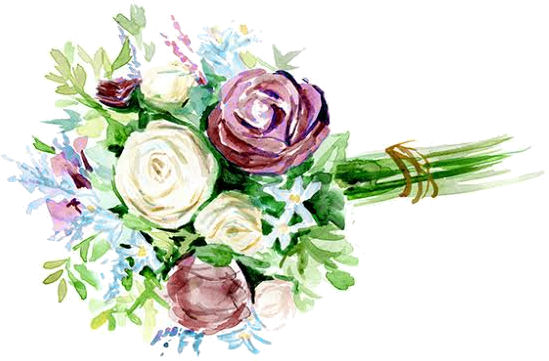
\includegraphics[width=0.45\textwidth]{graphics/flower.jpg}
\end{center}
